\documentclass[margin=0px]{article}

\usepackage{listings}
\usepackage[utf8]{inputenc}
\usepackage{graphicx}
\usepackage{float}
\usepackage[a4paper, margin=1in]{geometry}
\usepackage{subcaption}
\usepackage{amsthm}
\usepackage{amssymb}
\usepackage{amsmath}

\renewcommand{\figurename}{ábra}
\newenvironment{tetel}[1]{\paragraph{#1 \\}}{}
\newcommand{\R}{\mathbb{R}}

% A dokument itt kezdődik

\title{Záróvizsga tételsor \\ \large 14. Haladó algoritmusok}
\date{}
\author{Dobreff András}

\begin{document}
	\maketitle
	
	\begin{tetel}{Haladó algoritmusok}
			Gráfalgoritmusok: gráfok ábrázolás, szélességi bejárás, minimális költségű utak keresése, minimális költségű feszítőfa keresése, mélységi bejárás, DAG topologikus rendezése. Adattömörítések (Huffman- és LZW-algoritmus). Mintaillesztés módszerei.
	\end{tetel}
	
	\section{Gráfalgoritmusok}
		\subsection{Gráf ábrázolás}
			\begin{description}
				\item[Láncolt listás ábrázolás] \hfill \\
					A gráf csúcsait helyezzük el egy tömbben (vagy láncolt listában). Minden elemhez rendeljünk hozzá egy láncolt listát, melyben az adott csúcs szomszédjait (az esetleges élsúlyokkal) soroljuk fel. 
				\item[Mátrixos ábrázolás] \hfill \\
						Legyen a csúcsok elemszáma $n$. Ekkor egy $A^{n\times n}$ mátrixban jelöljük, hogy mely csúcsok vannak összekötve. Ekkor mind a sorokban, mind az oszlopokban a csúcsok szerepelnek, és az $a_{ij}$ cellában a $i$ csúcsból $j$ csúcsba vezető él súlya szerepel, ha nincs él a két csúcs között, akkor $-\infty$ (súlyozatlan esetben $1$ és $0$)
						
						Amennyiben a gráf irányítatlan nyilván $a_{ij} = a_{ji}$
			\end{description}
		\subsection{Szélességi bejárás}
			$G$ gráf (irányított/irányítatlan) $s$ startcsúcsából a távolság sorrendjében érjük el a csúcsokat. A legrövidebb utak feszítőfáját adja meg, így csak a távolság számít, a súly nem.
			
			A nyilvántartott csúcsokat egy sor adatszerkezetben tároljuk, az aktuális csúcs gyerekeit a sor-ba tesszük. A következő csúcs pedig a sor legelső eleme lesz.
			
			A csúcsok távolságát egy $d$, szüleiket egy $\pi$ tömbbe írjuk, és $\infty$ illetve $0$ értékekkel inicializáljuk.
			
			Az algoritmus:
			\begin{enumerate}
				\item Az $s$ startcsúcsot betesszük a sorba
				\item A következő lépéseket addig ismételjük, míg a sor üres nem lesz
				\item Kivesszük a sor legelső ($u$) elemét
				\item Azokat a gyerekcsúcsokat, melyeknek a távolsága nem $\infty$ figyelmen kívül hagyjuk (ezeken már jártunk)
				\item A többi gyerekre ($v$): beállítjuk a szülőjét ($\pi[v] = u$), és a távolságát ($d[v] = d[u]+1$). Majd berakjuk a sorba.
			\end{enumerate}
		\subsection{Minimális költségű utak keresése}
			\begin{description}
				\item[Dijkstra algoritmus] \hfill \\
					Egy $G$ irányított, pozitív élsúlyokkal rendelkező gráfban keres $s$ startcsúcsból minimális költségű utakat minden csúcshoz. 
					
					Az algoritmus a szélességi bejárás módosított változata. Mivel itt egy hosszabb útnak lehet kisebb a költsége, mint egy rövidebbnek, egy már megtalált csúcsot nem szabad figyelmen kívül hagyni. Ezért minden csúcs rendelkezik három állapottal (nem elért, elért, kész). A $d$ és $\pi$ tömböket a szélességi bejáráshoz hasonlóan kezeljük.
					
					A még nem kész csúcsokat egy prioritásos sorba helyezzük, vagy minden esetben minimumkeresést alkalmazunk.

				Az algoritmus:
				\begin{enumerate}
					\item Az $s$ startcsúcs súlyát 0-ra állítjuk eltároljuk
					\item A következő lépéseket addig ismételjük, míg a konténerünk üres nem lesz
					\item Kivesszük a sor legjobb ($u$) elemét, és "kész"-re állítjuk
					\item Ha egy gyerekcsúcs ($v$) nem kész, és a jelenleg hozzávezető út súlya kisebb, mint az eddigi, akkor: a szülőjét $u$-ra állítjuk ($\pi[v] = u$), és a súlyát frissítjük ($d[v] = d[u]+d(u,v)$).
					\item A többi csúcsot kihagyjuk.
				\end{enumerate}						
					
				\item[Bellman-Ford algoritmus] \hfill \\
					Egy $G$ élsúlyozott (akár negatív) irányított gráf $s$ startcsúcsából keres minden élhez minimális költségű utakat, illetve felismeri, ha negatív költségű kör van a gráfban. A $d$ és $\pi$ tömböket az előzőekhez hasonlóan kezeljük.
					
					Az algoritmus:
					\begin{enumerate}
						\item A startcsúcs súlyát állítsuk be 0-ra.
						\item $n-1$ iterációban menjünk végig az összes csúcson, és minden csúcsot ($u$) vessünk össze minden csúccsal ($v$). Ha olcsóbb utat találtunk akkor $v$-be felülírjuk a súlyát ($d[v] = d[u]+d(u,v)$), és a szülőjét ($\pi[v] = u$).
						\item Ha az $n$-edik iterációban is történt módosítás, negatív kör van a gráfban
					\end{enumerate}
			\end{description}
		\subsection{Minimális költség feszítőfa keresése}
			A Prim algoritmus egy irányítatlan élsúlyozott (akár negatív) gráf $s$ startcsúcsából keres minimális költségű feszítőfát. A $d$ és $\pi$ tömböket az előzőekhez hasonlóan kezeljük. Az algoritmus egy prioritásos sorba helyezi a csúcsokat.
			
			Az algoritmus:
			\begin{enumerate}
				\item A startcsúcs súlyát állítsuk be 0-ra.
				\item A csúcsokat behelyezzük a prioritásos sorba. 
				\item A következő lépéseket addig végezzük, míg a prioritásos sor ki nem ürül.
				\item Kiveszünk egy csúcsot ($u$) a sorból.
				\item Minden gyerekére ($v$), amely még a sorban és a nyilvántartott $v$-be vezető él súlya nagyobb, mint a most megtalált: A $v$ szülőjét $u$-ra változtatjuk, a nyilvántartott súlyt felülírjuk $d[v] = d(u,v)$. Majd felülírjuk a $v$ állapotát a prioritásos sorban.
				\item Azokkal a gyerekekkel, melyek nincsenek a sorban, vagy a súlyukon nem tudunk javítani, nem változtatunk.
			\end{enumerate}
		\subsection{Mélységi bejárás}
			$G$ irányított (nem feltétlenül összefüggő) gráf mélységi bejárásával egy mélységi fát (erdőt) kapunk. Az algoritmus a következő:
			\begin{itemize}
				\item Az élsúlyok nem játszanak szerepet
				\item Nincs startcsúcs, a gráf minden csúcsára elindítjuk az algoritmust. (Természetesen ekkor, ha már olyan csúcsot választunk, amin már voltunk, az algoritmus nem indul el.)
				\item A csúcsokat mohón választjuk, azaz minden csúcs gyerekei közül az elsőt választva haladunk előre, amíg csak lehet. (Olyan csúcsot találunk, amelynek nincs gyereke, vagy minden gyerekén jártunk már.)
				\item Ha már nem lehet előre haladni visszalépünk.
				\item Minden csúcshoz hozzárendelünk két értéket. Az egyik a mélységi sorszám, mely azt jelöli, hogy hanyadiknak értük el. A másik a befejezési szám, mely azt jelzi, hogy hanyadiknak léptünk vissza belőle. 
			\end{itemize}
			A gráf éleit a mélységi bejárás közben osztályozhatjuk. (Inicializáláskor minden értéket 0-ra állítottunk)
			\begin{itemize}
				\item Faél: A következő csúcs mélységi száma 0
				\item Visszaél: A következő csúcs mélységi száma nagyobb, mint 0, és befejezési száma 0 (Tehát az aktuális út egy előző csúcsára kanyarodunk vissza)
				\item Keresztél: A következő csúcs mélységi száma nagyobb, mint 0, és befejezési száma is nagyobb, mint 0, továbbá az aktuális csúcs mélységi száma nagyobb, mint a következő csúcs mélységi száma. (Ekkor egy az aktuális csúcsot megelőző csúcsból induló, már megtalált útba mutató éllel van dolgunk)
				\item Előreél: A következő csúcs mélységi száma nagyobb, mint 0, és befejezési száma is nagyobb, mint 0, továbbá az aktuális csúcs mélységi száma kisebb, mint a következő csúcs mélységi száma. (Ekkor egy az aktuális csúcsból induló, már megtalált útba mutató éllel van dolgunk)
			\end{itemize}
		\subsection{DAG Topologikus rendezése}
			\begin{description}
				\item[Alapfogalmak] \hfill
					\begin{itemize}
						\item Topologikus rendezés: \\
							Egy $G(V,E)$ gráf topologikus rendezése a csúcsok olyan sorrendje, melyben $\forall (u\rightarrow v) \in E$ élre $u$ előbb van a sorrendben , mint $v$
						\item DAG - Directed Acyclic Graph: \\
							Irányított körmentes gráf. \\
							Legtöbbször munkafolyamatok irányítására illetve függőségek analizálására használják.
							
							Tulajdonságok:
							\begin{itemize}
								\item Ha $G$ gráfra a mélységi bejárás visszaélt talál (Azaz kört talált) $\Longrightarrow$ $G$ nem DAG
								\item Ha $G$ nem DAG (van benne kör) $\Longrightarrow$ Bármely mélységi bejárás talál visszaélt
								\item Ha $G$-nek van topologikus rendezések $\Longrightarrow$ $G$ DAG
								\item Minden DAG topologikusan rendezhető.
							\end{itemize}
					\end{itemize} 
				\item[DAG topologikus rendezése] \hfill \\
					Egy $G$ gráf mélységi bejárása során tegyük verembe azokat a csúcsokat, melyekből visszaléptünk. Az algoritmus után a verem tartalmát kiírva megkapjuk a gráf egy topologikus rendezését.
			\end{description}
	\section{Adattömörítések}
		\subsection{Huffman-algoritmus}
			A Huffman-algoritmussal való tömörítés lényege, hogy a gyakrabban előforduló elemeket (karaktereket) rövidebb, míg a ritkábban előfordulókar hosszabb kódszavakkal kódoljuk.
			
			Ehhez tisztában kell lennünk az egyes karakterek gyakoriságával (vagy relatív gyakoriságával). Ezek alapján  egy ún. Huffman-fát építünk, melyben az éleket a kód betűivel címkézzük, a fa levelein a kódolandó betűk helyezkednek el, a gyökérből a levelekig vezető út címkéi alapján rajuk össze a kódszavakat.\\
			
			\noindent
			Az algoritmus (spec. bináris Huffman fára):
			\begin{enumerate}
				\item A kódolandó szimbólumokat gyakoriságaik alapján sorba rendezzük.
				\item A következő redukciós lépéseket addig hajtjuk végre, míg egy csoportunk marad.
				\item Kiválasztjuk az utolsó két elemet (legritkább), összevonjuk őket egy új csoportba, és ennek a csoportnak a gyakorisága a gyakoriságok összege lesz.
				\item A csoportot visszahelyezzük a rendezett sorba (gyakoriság alapján rendezve).
				\item A csoportból új csúcsot képezünk, mely csúcs az őt alkotó két elem szülője lesz. 
			\end{enumerate}
			
			\noindent
			Példa:\\
			Legyen a következő 5 betű, mely a megadott gyakorisággal fordul elő:\\
			
			\begin{tabular}{|c|c|c|c|c|}
				\hline A & B & C & D & E \\ 
				\hline 5 & 4 & 3 & 2 & 1 \\ 
				\hline 
			\end{tabular}\\
			
			 Ekkor a redukciós lépések a következők:
			 
			 \begin{itemize}
				\item \begin{tabular}{|c|c|c|c|}
				 	\hline A & B & C & D, E \\ 
				 	\hline 5 & 4 & 3 & 3 \\ 
				 	\hline 
				 \end{tabular}
			 
				 \item \begin{tabular}{|c|c|c|}
				 	\hline C, D, E & A & B \\ 
				 	\hline 6 & 5 & 4\\ 
				 	\hline 
				 \end{tabular}
				 
				 \item \begin{tabular}{|c|c|}
				 	\hline A , B & C, D, E\\ 
				 	\hline 9 & 6\\ 
				 	\hline 
				 \end{tabular}
				 
				 \item \begin{tabular}{|c|}
				 	\hline A , B , C, D, E\\ 
				 	\hline 15\\ 
				 	\hline 
				 \end{tabular}
			\end{itemize}  
			
			A huffman-fa a XY. ábrán látható.
			
			\begin{figure}[H]
				\centering
				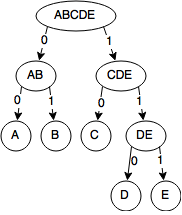
\includegraphics[width=0.3\textwidth]{img/Huffman_fa.png}
				\caption{Huffman-fa példa}
				\label{fig:Huffman_fa}
			\end{figure}
			
			Tehát a kódszavak:
			
			\begin{tabular}{|c|c|c|c|c|}
				\hline A & B & C & D & E \\ 
				\hline 00 & 01 & 10 & 110 & 111 \\ 
				\hline 
			\end{tabular} 
		\subsection{LZW-algoritmus}
			Az LZW (Lempel-Ziv-Welch) tömörítésnek a lényege, hogy egy szótárat bővítünk folyamatosan, és az egyes kódolandó szavakhoz szótárindexeket rendelünk.
			\begin{description}
				\item[Kódolás] \hfill \\
					A kódolás algoritmusa a következő lépésekből áll:
					 \begin{enumerate}
					 	\item A szótárt inicializáljuk az összes 1 hosszú szóval
					 	\item \label{itm:szotar} Kikeressük a szótárból a leghosszabb, jelenlegi inputtal összeillő $W$ sztringet
					 	\item $W$ szótárindexét kiadjuk, és $W$-t eltávolítjuk az inputról
					 	\item A $W$ szó és az input következő szimbólumának konkatenációját felvesszük a szótárba
					 	\item A \ref{itm:szotar}. lépéstől ismételjük
					 \end{enumerate}
				\item[Dekódolás] \hfill \\
					A dekódolás során is építenünk kell a szótárat. Ezt már azonban csak a dekódolt szöveg(rész) segítségével tudjuk megtenni, mivel egy megkapott kód dekódolt szava és az utána lévő szó első karakteréből áll össze a szótár következő eleme. 
					
					Tehát a dekódolás lépései:
					\begin{enumerate}
					\item Kikeressük a kapott kódhoz tartozó szót a szótárból ($u$), az output-ra rakjuk
					\item Kikeressük a következő szót ($v$) a szótárból, az első szimbólumát $u$-hoz konkatenálva a szótárba rakjuk a következő indexszel.
					\item Amennyiben már nincs következő szó, dekódolunk, de nem írunk a szótárba.
					\end{enumerate}
					
					Megtörténhet az az eset, hogy mégis kapunk olyan kódszót, mely még nincs benne a szótárban. Ez akkor fordulhat elő, ha a kódolásnál az aktuálisan szótárba írt szó következik.\\
					
					Példa:
					
					Szöveg: AAA\\
					Szótár: A - 1
					
					Ekkor a kódolásnál vesszük az első karaktert, a szótárbeli indexe 1, ezt kiküldjük az outputra. A következő karakter A, így AA-t beírjuk a szótárba 2-es indexszel. Az első karaktert töröljük az inputról. Addig olvasunk, míg szótárbeli egyezést találunk, így AA-t olvassuk (amit pont az előbb raktunk be), ennek indexe 2, tehát ezt küldjük az outputra. AA-t töröljük az inputról, és ezzel végeztünk is. Az output: 1,2
					
					Dekódoljuk az 1,2 inputot! Jelenleg a szótárban csak A van 1-es indexszel. Vegyük az input első karakterét, az 1-et, ennek szótárbeli megfelelője A. Ezt tegyük az outputra. A következő index a 2, de ilyen bejegyzés még nem szerepel a szótárban. \\
					
					Ebben az esetben a dekódolásnál, egy trükköt vetünk be. A szótárba írás pillanatában még nem ismert a beírandó szó utolsó karaktere (A példában A-t találtuk, de nem volt 2-es bejegyzés). Ekkor ?-et írunk a szótárba írandó szó utolsó karakterének helyére. (Tehát A? - 2 kerül a szótárba). De mostmár tudni lehet az új bejegyzés első betűjét ( A? - 2 az új bejegyzés, ennek első betűje A). Cseréljük le a ?-et erre a betűre. (Tehát AA - 2 lesz a szótárban).
			\end{description}
	\section{Mintaillesztés}
		\subsection{Knuth-Morris-Pratt algoritmus}
			A Knuth-Morris-Pratt eljárásnak a Brute-Force (hasonlítsuk össze, toljunk egyet, stb..) módszerrel szemben az az előnye, hogy egyes esetekben, ha a mintában vannak ismétlődő elemek, akkor egy tolásnál akár több karakternyit is ugorhatunk.
			
			\begin{figure}[H]
				\centering
				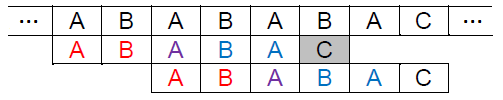
\includegraphics[width=0.4\textwidth]{img/KMP_sample.png}
				\caption{KMP algoritmus több karakter tolás estén}
				\label{fig:KMP_sample}
			\end{figure}
			
			Az ugrás megállapítását a következőképp tesszük: Az eddig megvizsgált egyező mintarész elején (prefix) és végén (suffix) olyan kartersorozatot keresünk, melyek megegyeznek. Ha találunk ilyet, akkor a mintát annyival tolhatjuk, hogy az elején lévő része ráilleszkedjen a végén levőre.
			
			Azt, hogy ez egyes esetekben mekkorát tolhatunk nem kell minden elromlás alkalmával vizsgálni. Ha a mintára önmagával lefuttatjuk az algoritmus egy módosított változatát (\ref{fig:KMP_initnext}. ábra), kitölthetünk egy tömböt, mely alapján a tolásokat végezni fogjuk.
			
			\begin{figure}[H]
				\centering
				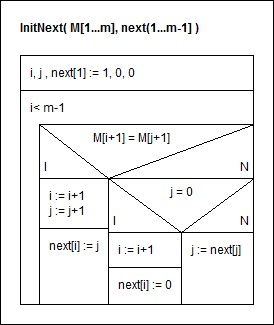
\includegraphics[width=0.3\textwidth]{img/KMP_initnext.jpg}
				\caption{KMP tolásokat szabályzó tömb kitöltése}
				\label{fig:KMP_initnext}
			\end{figure}
			
			Az algoritmus (ld \ref{fig:KMP}. ábra):
			\begin{itemize}
				\item Két indexet $i$ és $j$ futtatunk a szövegen illetve a mintán.
				\item Ha az $i+1$-edik és $j+1$-edik karakterek megegyeznek, akkor léptetjük mind a kettőt.
				\item Ha nem egyeznek meg, akkor:
					\begin{itemize}
						\item Ha a minta első elemét vizsgáltuk, akkor egyet tolunk a mintán, magyarul a minta indexe marad az első betűn, és a szövegben lévő indexet növeljük eggyel ($i=i+1$)
						\item Ha nem a minta első elemét vizsgáltuk, akkor annyit tolunk, amennyit szabad. Ez azt jelenti, hogy csak a mintán lévő indexet helyezzük egy kisebb helyre ($j = next[j]$)
					\end{itemize}
				\item Addig megyünk, míg vagy a minta, vagy a szöveg végére nem érünk. Ha a minta végére értünk, akkor megtaláltuk a mintát a szövegben, ha a szöveg végére értünk, akkor pedig nem.
			\end{itemize}
			
			\begin{figure}[H]
				\centering
				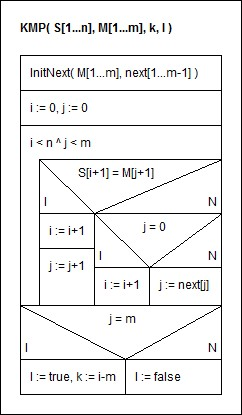
\includegraphics[width=0.3\textwidth]{img/KMP.jpg}
				\caption{KMP algoritmus}
				\label{fig:KMP}
			\end{figure}
		\subsection{Boyer-Moore  | Quick search algoritmus}
			Míg a KMP algoritmus az elromlás helye előtti rész alapján döntött a tolásról, addig a QS a minta utáni karakter alapján. Tehát elromlás esetén:
			\begin{itemize}
				\item Ha a minta utáni karakter benne van a mintában, akkor jobbról az első előfordulására illesztjük. (\ref{fig:BoyerMoore_shift1}. ábra)
				\begin{figure}[H]
					\centering
					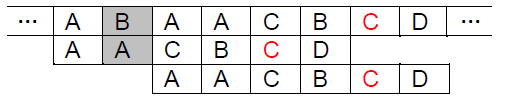
\includegraphics[width=0.4\textwidth]{img/BoyerMoore_shift1.png}
					\caption{QS - eltolás ha a minta utáni karakter benne van a mintában}
					\label{fig:BoyerMoore_shift1}
				\end{figure}
				\item Ha a minta utáni karakter nincs benne a mintában, akkor a mintát ezen karakter után illesztjük. (\ref{fig:BoyerMoore_shift2}. ábra)
				\begin{figure}[H]
					\centering
					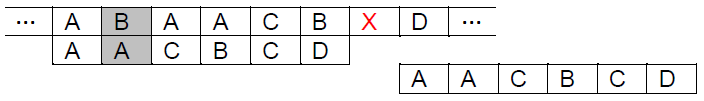
\includegraphics[width=0.6\textwidth]{img/BoyerMoore_shift2.png}
					\caption{QS - eltolás ha a minta utáni karakter nincs benne a mintában}
					\label{fig:BoyerMoore_shift2}
				\end{figure}
			\end{itemize}
			
			Az eltolás kiszámítását megint elő lehet segíteni egy tömbbel, most azonban, mivel nem a minta az érdekes, és nem tudjuk pontosan mely karakterek szerepelnek a szövegben, így a tömbbe az egész abc-t fel kell vennünk (\ref{fig:BoyerMoore_initshift}. ábra)
			
			\begin{figure}[H]
				\centering
				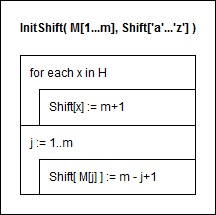
\includegraphics[width=0.3\textwidth]{img/BoyerMoore_initshift.jpg}
				\caption{QS - Az eltolást elősegítő tömb ($Shift['a'...'z']$) konstruálása}
				\label{fig:BoyerMoore_initshift}
			\end{figure}
			
			Az algoritmus (ld. \ref{fig:BoyerMoore}. ábra):
			\begin{itemize}
				\item Két indexet $k$ és $j$ futtatunk a szövegen illetve a mintán.
				\item Ha a szöveg $k+j$-edik eleme megegyezik a minta $j$-edik karakterével, akkor léptetjük $j$-t (mivel a szövegben $k+j$-edik elemet nézzük, így elég $j$-t növelni).
				\item Ha nem egyeznek meg, akkor:
				\begin{itemize}
					\item Ha a minta már a szöveg végén van ($k=n-m$), akkor csak növeljük $k$-t eggyel, ami hamissá teszi a ciklus feltételt.
					\item Ha még nem vagyunk a szöveg végén $k$-t toljuk annyival, amennyivel lehet (ezt az előre beállított $Shift$ tömb határozza meg). És a $j$-t visszaállítjuk 1-re.
				\end{itemize}
				\item Addig megyünk, míg vagy a minta végére érünk $j$-vel, vagy a mintát továbbtoltuk a szöveg végénél. Előbbi esetben egyezést találtunk, míg az utóbbiban nem.
			\end{itemize}
			
			\begin{figure}[H]
				\centering
				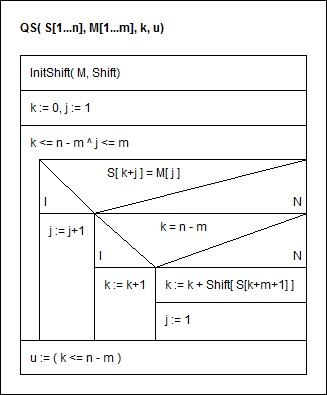
\includegraphics[width=0.4\textwidth]{img/BoyerMoore.jpg}
				\caption{QS}
				\label{fig:BoyerMoore}
			\end{figure}
		\subsection{Rabin-Karp algoritmus}
			A Rabin-Karp algoritmus lényege, hogy minden betűhöz az ábécéből egy számjegyet rendelünk, és a keresést számok összehasonlításával végezzük. Világos, hogy ehhez egy ábécé méretnek megfelelő számrendszerre lesz szükségünk. A szövegből mindig a minta hosszával egyező részeket szelünk ki, és ezeket hasonlítjuk össze.\\
			
			\noindent
			Példa:\\
				Minta: BBAC $\rightarrow$ 1102 \\
				Szöveg: DACABBAC $\rightarrow$ 30201102, amiből a következő számokat állítjuk elő: 3020, 0201, 2011, 0110, 1102\\
			
			\noindent
			A fent látható szeletek lesznek az $s_i$-k.\\
			
			\noindent
			Az algoritmus működéséhez azonban számos apró ötletet alkalmazunk:
			\begin{enumerate}
				\item A minta számokká alakítását Horner-módszer segítségével végezzük.
					\begin{figure}[H]
						\centering
						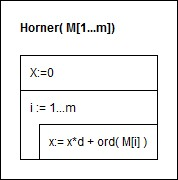
\includegraphics[width=0.3\textwidth]{img/RK_Horner.jpg}
						\caption{RK - Horner-módszer}
						\label{fig:RK_Horner}
					\end{figure}
					Az $ord()$ függvény az egyes betűknek megfelelő számot adja vissza. A $d$ a számrendszer alapszáma.
				\item A szöveg mintával megegyező hosszú szeleteinek ($s_i$) előállítása: \\
					$s_0$-t a Horner-módszerrel ki tudjuk számolni. Ezek után $s_{i+1}$ a következőképp számolandó:
					\[s_{i+1} = (s_i - ord(S[i])\cdot d^{m-1})\cdot d  + ord(S[i+1])\]
					\textit{Magyarázat: $s_i$ elejéről levágjuk az első számjegyet ($s_i - ord(S[i])\cdot d^{m-1}$), majd a maradékot eltoljuk egy helyiértékkel (szorzás $d$-vel), végül az utolsó helyiértékre beírjuk a következő betűnek megfelelő számjegyet ($+ord(S[i+1])$)}
					
					Példa:
					
						Az előző példa szövegével és mintájával ($d=10$ elemű ábécé és $m=4$ hosszú minta): \\
							$s_0 = 3020$, ekkor: $s_{0+1} = s_1 = (3020 - ord(D) \cdot 10^3)\cdot 10 + ord(B) = (3020-3000)\cdot 10 +1 = 0201$
				\item Felmerülhet a kérdés, hogy az ilyen magas alapszámú számrendszerek nem okoznak-e gondot az ábrázolásnál? A kérdés jogos. Vegyük a következő életszerű példát:
				
				4 bájton ábrázoljuk a számainkat ($2^{32}$). Az abc legyen 32 elemű ($d=32$), a minta 8 hosszú ($m=8$). Ekkor a $d^{m-1}$ kiszámítása: $32^7 = (2^5)^7 = 2^{35}$ , ami már nem ábrázolható 4 bájton.
				
				Ennek kiküszöbölésére vezessünk be egy nagy $p$ prímet, melyre $d\cdot p$ még ábrázolható. És a műveleteket számoljuk $\mod{p}$. Ekkor természetesen a kongruencia miatt lesz olyan eset, amikor az algoritmus egyezést mutat, mikor valójában nincs. Ez nem okoz gondot, mivel ilyen esetben karakterenkénti egyezést vizsgálva ezt a problémát kezelni tudjuk. (Fordított eset nem fordul elő tehát nem lesz olyan eset, mikor karakterenkénti egyezés van, de numerikus nincs). [Ha $p$ kellően nagy, a jelenség nagyon ritkán fordul elő.]
				
				\item A $\mod{p}$ számítás egy másik problémát is felvet. Ugyanis a kivonás alkalmával negatív számokat is kaphatunk.
				
				Például: Legyen $p=7$, ekkor, ha $ord(S[i]) = 9$, akkor előző számítás után $s_i = 2...$, de ebből $ord(S[i])\cdot d^{m-1} = 9\cdot 10^3 = 9000$-et vonunk ki negatív számot kapunk. 
				
				Megoldásként $s_{i+1}$-et két lépésben számoljuk:
				\[s := (s_i+d\cdot p - ord(S[i])\cdot d^{m-1}) \mod{p} \]
				\[s_{i+1} := (s\cdot d + ord(S[i+1])) \mod{p} \]
			\end{enumerate}			
			A fentiek alapján az algoritmus a következő (ld. \ref{fig:RK}. ábra)
			\begin{enumerate}
				\item Kiszámoljuk $d^{m-1}$-et ($dm1$)
				\item Egy iterációban meghatározzuk Horner-módszerrel a minta számait ($x$) és $s_0$-t
				\item Ellenőrizzük, hogy egyeznek-e
				\item Addig számolgatjuk $s_i$ értékét míg a minta nem egyezik $s_i$-vel, vagy a minta a szöveg végére nem ért.
			\end{enumerate}
			\begin{figure}[H]
				\centering
				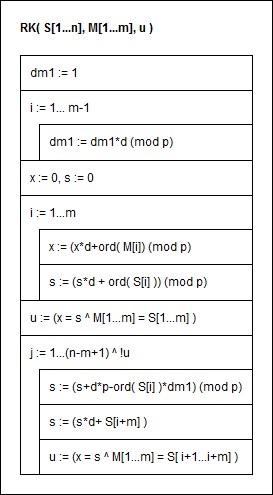
\includegraphics[width=0.3\textwidth]{img/RK.jpg}
				\caption{RK}
				\label{fig:RK}
			\end{figure}
\end{document}